\documentclass[12pt,a4paper]{article}

% =========================================
% PAGE SETUP
% =========================================
\usepackage[
    a4paper,
    margin=25.4mm
]{geometry}


% =========================================
% BASIC PACKAGES
% =========================================
\usepackage{graphicx}       % Images
\usepackage{amsmath}        % Mathematics
\usepackage{amssymb}        % Mathematical symbols
\usepackage{booktabs}       % Professional tables
\usepackage{float}          % [H] figure/table positioning
\usepackage{caption}        % Caption customization
\usepackage{hyperref}       % Hyperlinks and references
\usepackage{ragged2e}       % Text alignment
\usepackage{setspace}       % Line spacing
\usepackage{pdflscape}      % Landscape mode
\usepackage{hyperref}       % Clickable links and references
\usepackage{array}          % Customized tables
\usepackage{tabularx}
% =========================================
% APA REFERENCING
% =========================================

\usepackage[
    style=apa,
    backend=biber
]{biblatex}

\addbibresource{references.bib}


% =========================================
% HYPERLINK SETTINGS
% =========================================
\hypersetup{
    colorlinks=true,
    linkcolor=black,
    urlcolor=black,
    citecolor=black,
    pdftitle={Critical Research Review Article}
}

% Table and figure caption formatting
\DeclareCaptionFont{captionnine}{\fontsize{9pt}{11pt}\selectfont}

\captionsetup[table]{
    font=captionnine,
    justification=raggedright,
    singlelinecheck=false,
    labelsep=colon
}

\captionsetup[figure]{
    font=captionnine,
    justification=centering,
    singlelinecheck=false,
    labelsep=colon
}


% =========================================
% DOCUMENT
% =========================================
\begin{document}
\begin{center}

\includegraphics[width=0.45\textwidth]{figures\mmu_logo.png}\\[1.5cm]
{\fontsize{18}{22}\selectfont\textbf{CRITICAL RESEARCH REVIEW ARTICLE}}

\vspace{0.5cm}

{\fontsize{18}{22}\selectfont\textbf{THE ROLE OF DIGITAL FORENSICS IN CYBERCRIME INVESTIGATIONS}}

\vspace{1cm}

{\fontsize{12}{14}\selectfont\textbf{Group Members}}

\vspace{0.3cm}

{\fontsize{12}{14}\selectfont
1. Wan Wei Siang -- 251UC2508W\\
2. Elsa Zara Binti Fakhurrazi -- 251UC2502P\\
3. Student Name -- Student ID\\
4. Student Name -- Student ID
}

\vspace{0.8cm}

{\fontsize{12}{14}\selectfont
\textbf{Programme:} Research Method\\
\textbf{Course:} CPT6123\\
\textbf{Lecturer:} Rohana Binti Mydin\\
\textbf{Semester:} 2620\\
\textbf{Submission Date:} 6th September 2026
}

\end{center}


% =========================================
% ABSTRACT
% =========================================

\vspace{0.5cm}

\noindent
\textbf{Abstract}

\vspace{0.2cm}

\begin{justify}

Write a concise summary of the entire review article. Write a concise summary of the entire review article. Write a concise summary of the entire review article. Write a concise summary of the entire review article.

Write a concise summary of the entire review article.Write a concise summary of the entire review article.Write a concise summary of the entire review article.



The abstract should include:

\begin{itemize}
    \item Background/context of the selected research topic
    \item Purpose of the review
    \item General approach used to select and analyse the research articles
    \item Major findings from the reviewed literature
    \item Key research gaps identified
    \item Overall conclusion
\end{itemize}

\textbf{Recommended length: 150--250 words.}

\vspace{0.3cm}

\textbf{Keywords:} Digital Forensics; Cybersecurity; Investigation; Multimedia forensics; Cybercrime; Biometric; Data privacy

\end{justify}




% =========================================
% TABLE OF CONTENTS
% =========================================

\newpage

\tableofcontents

\newpage



% =========================================
% MAIN CONTENT
% =========================================

\begin{justify}

% =========================================
% 1. INTRODUCTION
% =========================================

\section{Introduction}

\subsection{Background}

As digital technology has experienced rapid evolution and expansion throughout the years, it has slowly integrated itself into most aspects of our own lives, from communications to our governance. Naturally, this boon that provides us convenience and connectivity will bring upon malicious actors that will misuse them to commit cybercrimes, ranging from small scaled crimes like identity theft and cybertheft of financial and card payment data to much larger scale ones such as cyberespionage and ransomware attacks.

As such, traditional methods of investigation have been proven to be ineffective in combating and solving these crimes. Hence, digital forensics as a discipline has seen a rise within the fields of cybersecurity and law enforcement to ensure that the malicious actors will have their deserved justice dealt to them alongside learning their methods to better suppress the surge of cybercrime.


% Introduce the selected research topic and explain why it is important.

% This is how you add inline references in the document given that all your references have been copied in the references.bib.
% Recent studies have demonstrated the effectiveness of artificial
% intelligence techniques %\parencite{smith2024}.

% Follow this example to include more than one references.Several studies have investigated these approaches
% %\parencite{smith2024,lee2023,ahmad2022}.

% \vspace{0.5cm}
% Discuss:

% \begin{itemize}
%     \item What is the research topic?
%     \item What problem does it address?
%     \item Why is the problem important?
%     \item Where is the topic currently being applied?
%     \item Why is there a need to study/review this topic?
% \end{itemize}

% Students should support important statements with appropriate research references.


\subsection{Problem Statement}

\vspace{0.5cm}
Almost every part of daily life now runs through a computer or a phone, and crime has followed right along with it. Money gets stolen, systems get broken into, and all of it can happen from the other side of the world. Digital forensics — the work of digging through devices and networks for proof of what happened — has become central to how law enforcement operates. That said, the field is under real strain right now.

For a long time, the basic strategy was straightforward: keep a list of known bad signatures and block anything that matched. That worked fine when attackers were unsophisticated. They aren't anymore. Advanced Persistent Threats, for example, are designed to slip past defenses and remain undiscovered for lengthy periods of time, silently removing important data from a network without raising any alarms. The scope of the problem is difficult to overestimate – cybercrime is expected to cost the global economy 10.5 trillion dollars by 2025, yet discovery is sometimes excruciatingly slow: one research estimated that the average time to find a breach was 212 days.


Part of the difficulty stems from the fact that digital forensics is a collection of disparate fields. Network forensics works with traffic, mobile forensics with phones and tablets, and then there's cloud, database, IoT, and multimedia forensics , each with its own set of tools and standards. A case that involves more than one of these areas requires investigators to piece together methodologies that were never intended to function together, slowing things slowly and introducing opportunity for mistake .


Criminals aren't making this easier, either. Encryption scrambles communications. Steganography hides malicious code inside what looks like an ordinary image. Fileless virus operates totally in memory and leaves no trace when the system reboots. Some players are even using blockchain to hide their actions. Even when investigators uncover anything, it does not always make it to court – shoddy paperwork, uneven processes, and contradicting legislation across jurisdictions are major reasons solid evidence is tossed out.


Artificial intelligence is frequently presented as the solution. It's easy to see why: machine learning is genuinely good at finding patterns buried in massive datasets and flagging behavior that a human analyst might miss , and there's evidence that AI-powered tools outperform older methods in terms of detection rate and false positives . But AI brings its own baggage. These models are frequently black boxes, so it's not always clear why a system flagged what it flagged. They can be manipulated with carefully designed adversarial inputs. They require massive training datasets, which are not always accessible, as well as significant computational capacity to function.


Then there's the smart-device problem. Homes are full of smart speakers, locks, thermostats, TVs; factories run thousands of interconnected sensors. All of this results in a massive, jumbled volume of data in inconsistent forms, dispersed among devices, cloud servers, and local storage. Figuring out where the relevant evidence even lives, let alone extracting it and proving it hasn't been tampered with, is genuinely difficult in this kind of distributed environment.


The legal landscape doesn't help. Privacy laws vary greatly by country; some countries openly share evidence while others do not, and permissible investigation tactics range from one another. Investigators must operate within this patchwork while adhering to guidelines such as GDPR and CCPA, and a misstep here might torpedo a case completely.


Despite years of research in this area, there is still no cohesive method that tackles all of these issues simultaneously. Standardized testing techniques for forensic tools are sparse, multi-domain datasets are scarce, and technologies produced by various manufacturers frequently do not work together. Furthermore, new dangers such as deepfakes and adversarial assaults continue to emerge and necessitate their own solutions.

\subsection{Objectives of the Review}

%State the objectives of the review article.

This study aims to assess where digital forensics is today: what has been solved, what has not, and where the profession appears to be headed — with a focus on how AI and similar technologies might boost investigations and protect evidence integrity.


More specifically:


First, we look at current practice in six domains: network, mobile, database, IoT, cloud, and multimedia forensics, highlighting the key issues, the tools and methodologies used, and the largest gaps in each.


Second, we evaluate how well AI-based methods function in practice, focusing on deep learning, federated learning, and anomaly detection to identify where these approaches succeed and where they fail .


Third, we examine the problems provided by new threats such as APTs, encryption, anti-forensic tactics, steganography, and AI-generated media, as well as potential responses .


Fourth, we look at the legal and ethical frameworks that shape the field, such as how courts assess the admissibility of digital evidence, chain-of-custody requirements, privacy protections, and the challenges that come with cross-border investigations.


Fifth, we present a cross-domain framework that combines federated learning with context-aware policy enforcement, which is intended to function across hybrid cloud, IoT, and corporate contexts while addressing the constraints of current single-domain techniques.


Finally, we highlight areas for future research, including explainable AI, quantum-resistant encryption, blockchain-based evidence tracking, privacy-preserving threat intelligence sharing, and automated attack attribution.



\subsection{Research Questions}

%Develop 2--4 research questions that guide the review.

\vspace{0.2cm}

\textbf{RQ1:} What are the predominant methodologies and tools used in cybercrime investigations?

\vspace{0.2cm}

\textbf{RQ2:} What are the implications of artificial intelligence use in digital forensics?

\vspace{0.2cm}

\textbf{RQ3:} What are the methodological limitations identified in the current studies on digital forensics?

\vspace{0.2cm}

\textbf{RQ4:} What areas of digital forensics warrant further research?


% =========================================
% 2. REVIEW METHODOLOGY
% =========================================

\section{Review Methodology}

Explain how the group conducted the literature review.


\subsection{Literature Search Strategy}

%Describe:
To ensure the analysis we conducted are within the scope of our research and provides comprehensive depth, it is imperative to employ necessary techniques and paper selection for proper evaluation.

Firstly, a simple protocol was followed when selecting papers such that it is sourced explicitly using from trusted sources such as IEEE Xplore, ScienceDirect, IAES International Journal, arXiv, NUML International Journal. These academic databases were chosen for their viability to be cited, their coverage and for their contributions to digital forensics in cybersecurity. 

A combination of keywords were used as search terms such as “digital forensics,” “cybersecurity,” “investigation,” “artificial intelligence in digital forensics.” These words along with “AND” and “OR” boolean operators used to refine the search and identify available and relevant papers. 

Once the search had narrowed, papers were selected based on an initial screening based on title relevance to our subject, and were viewed in full-text to skim through its content. 

Following the compilation of papers, an inclusion and exclusion criteria were used to determine whether it would be included or discarded.

% Example databases:

% \begin{itemize}
%     \item Scopus
%     \item Web of Science
%     \item IEEE Xplore
%     \item ScienceDirect
%     \item SpringerLink
%     \item ACM Digital Library
%     \item Google Scholar
% \end{itemize}

\subsection{Inclusion and Exclusion Criteria}

% Describe the criteria used to determine which research articles were included in or excluded from the review.
To ensure the selection of research articles are of high quality and relevant to our research, a systematic inclusion and exclusion criteria were followed strictly.

\textbf{Inclusion criteria:}

\begin{enumerate}
    \item Relevance: The paper must continuously be relevant to the current subject and contains at least one aspect of digital forensics. 
    \item Publication Date: Published between 2021 and 2026 to ensure that the studies discussed are updated and reflect current issues.
    \item Page Length: Its pages were a minimum of 6 pages in length to ensure wide depth coverage on the subject. 
    \item Accessibility: The full-text is available at all times to be viewed for proper analysis.
    \item Complete Information: Bibliographic information are complete and readily available for proper citation and referencing.
    \item Coverage: The coverage of its subject is diversified and allows for new research areas to develop.
    \item Research Contribution: the studies must have its own original findings through experiments or have a concise discussion related to digital forensics.
\end{enumerate}

\textbf{Exclusion criteria:}

\begin{enumerate}
    \item Published before the year 2021.
    \item Page length is less than 6 pages. 
    \item Full-text is not readily available to view. 
    \item Insufficient bibliographic information for proper referencing.
    \item Its research methodology is not readily disclosed and transparent. 
    \item Its title relevance to our subject were determined out-of-scope. 
    \item In a language other than English.
    % \item Duplicate publications
    % \item Non-peer-reviewed publications
    % \item Articles outside the selected publication period
    % \item Articles without sufficient methodological or research information
\end{enumerate}

\end{justify}

% =========================================
% SAMPLE TABLE
% =========================================

% \begin{table}[H]
% \caption{Inclusion and exclusion criteria used for the literature review}
% \label{tab:inclusion-exclusion}

% \fontsize{10pt}{12pt}\selectfont

% \begin{tabular}{|p{4cm}|p{5cm}|p{5cm}|}
% \hline
% \centering\textbf{Criteria} &
% \centering\textbf{Inclusion} &
% \centering\textbf{Exclusion}
% \tabularnewline
% \hline

% \centering Publication type &
% \centering Peer-reviewed research articles &
% \centering Non-peer-reviewed articles
% \tabularnewline
% \hline

% \centering Publication period &
% \centering [e.g., 2021--2026] &
% \centering Articles outside selected period
% \tabularnewline
% \hline

% \centering Language &
% \centering English &
% \centering Other languages
% \tabularnewline
% \hline

% \centering Topic &
% \centering Directly related to selected topic &
% \centering Not directly related
% \tabularnewline
% \hline

% \centering Full text &
% \centering Full-text available &
% \centering Full text unavailable
% \tabularnewline
% \hline

% \end{tabular}

% \end{table}

% This is a sample table. Tables should be placed in the main text near to the first time they are cited, with the caption on top and left aligned. The font of the table caption is size 9 and the content in the table is size 10.



% =========================================
% SAMPLE FIGURE
% =========================================

% \begin{figure}[H]
%     \centering

%     \fbox{%
%         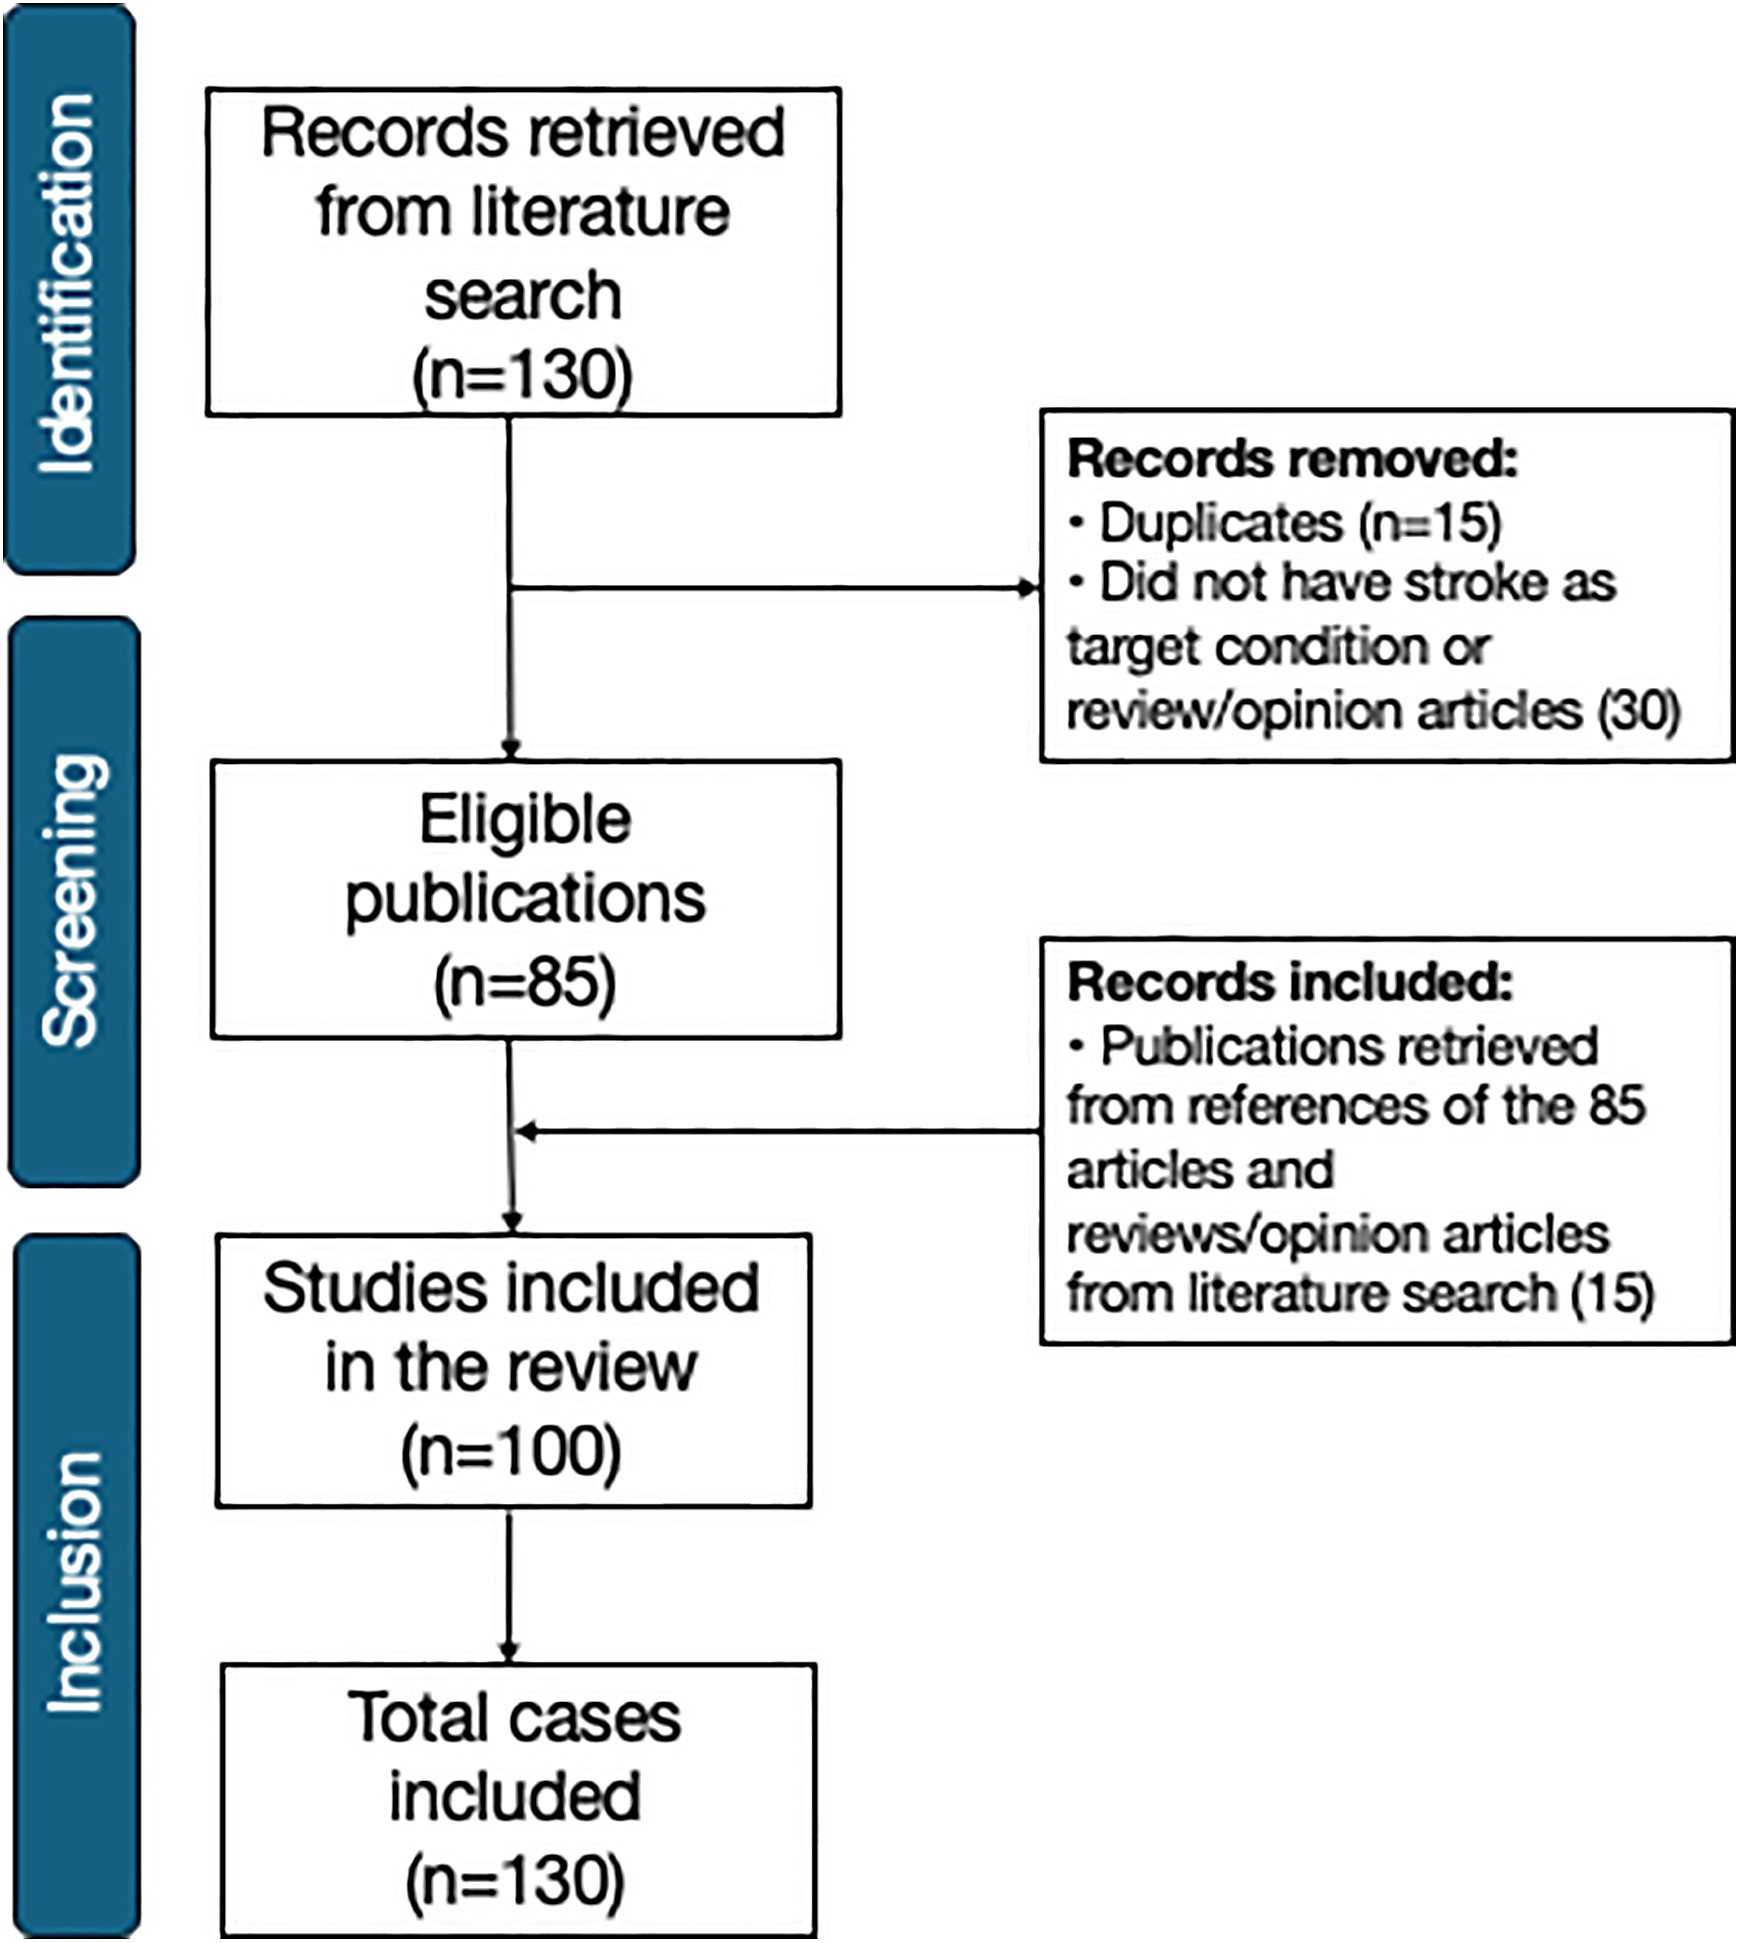
\includegraphics[width=0.80\textwidth]{figures/Prisma.jpg}%
%     }

%     \caption{PRISMA flow diagram of the study selection process.}
%     \label{fig:prisma}
% \end{figure}


% This is a figure. All figures should be centred with figure caption following the sequence Figure 1, Figure 2, and so on. The caption should also be centred. The caption for figures should be size 9.



\subsection{Article Selection}

Following the initial compilation of research articles through title relevance, papers were rejected based on its page length being less than 6 pages, its publishing before 2021, and its insufficient research, amongst others. 

Once compiled, each paper was meticulously examined through abstract inspection and the content of the main body’s key findings and points. Concluding the article selection, 12 papers were selected based on the viability of adhering to the inclusion and exclusion criteria and was taken for literature review and further analysis.

% Each student must review \textbf{at least 3 research articles}.

% Therefore:

% \begin{itemize}
%     \item \textbf{Minimum articles per student = 3}
%     \item \textbf{Minimum articles per group = 12}
% \end{itemize}

% The group may use more than 12 articles if necessary.

% Explain how the final articles were selected for the review.




% =========================================
% 3. LITERATURE REVIEW
% =========================================

\section{Literature Review}

\subsection{Theme 1: Standardised Practices and Advancements of Digital Forensics}

Through the rampant evolution of cybercrime in its sophistication of execution alongside the current digital age allowing access for various methods to execute cybercrime, digital forensics as a field within computer science has gone through many advancements to ensure that cybercriminals will face their due justice. 

To better evaluate Digital Forensic’s role in investigating and solving cybercrime, it would be apt to first understand the standardised methods of which the practitioners of digital forensics utilise in order to obtain the proper digital evidence for the committed cybercrime, and then delve into the various advancements made towards improving digital forensics' own practices as a whole.

Table 2 showcases research articles which align with the current theme of Standardised Practices of Digital Forensics, alongside their methodologies of research.

\begin{table}[H]
\caption{Research Articles for Standardised Practices of Digital Forensics and their Methodology}
\label{tab:inclusion-exclusion}

\fontsize{10pt}{12pt}\selectfont

\begin{tabular}{|p{4cm}|p{5cm}|p{5cm}|}
\hline
\centering\textbf{Research Articles} &
\centering\textbf{Primary Objectives} &
\centering\textbf{Methodology}
\tabularnewline
\hline

\centering \cite{ilyas2024role}  &
\centering To analyze the extent and legal strength of digital forensic evidence within the Indonesian legal system. &
\centering \textbf{Normative}: Viewing law as a system of norms. Utilises philosophical (Nature of digital forensics), conceptual (Test and analyse concepts), and case (study and analyze electronic crime cases) approaches.
\tabularnewline
\hline

\centering \cite{hassan2025}  &
\centering To evaluate the effectiveness of current digital forensic strategies and the possibility of enhancing them &
\centering \textbf{Qualitative}: Comparative analysis of digital forensic tools alongside examination of high-profile cybercrime case studies.
\tabularnewline
\hline

\centering \cite{sharma2024digital} &
\centering To investigate the adherence to legal standards and reporting procedures in forensic investigations. &
\centering \textbf{Quantitative Content Analysis}: 
Literature review of 40 reports from a quasi-experiment
\tabularnewline
\hline

\centering \cite{ARIF2025104296}  &
\centering To evaluate the challenges of digital forensics the existing methodologies face &
\centering \textbf{Systematic Literature Review (SLR)}: Analysis of peer-reviewed publications from 2019 to 2025 across prominent databases.
\tabularnewline
\hline

\end{tabular}

\end{table}

\subsubsection{Comparison of Research Objectives and Scope}

The chosen research articles intends to explore the transformation of digital forensics from traditional reactive models to much more reactive and intelligent frameworks.

\begin{itemize}
    \item \textbf{General Evolution and AI Integration} : Research by \cite{vaddi2024enhancements} focuses on the evolution of digital forensics over the past five years, specifically aiming to provide a high-level overview of AI’s potential to solve modern difficulties. Their objective is to guide developers in constructing intelligent, automated tools for effective crime detection across blockchain, cloud, and deep learning (DL) domains \cite{vaddi2024enhancements}.
    \item \textbf{Smart Environments and Forensic Readiness}: \cite{alenezi2023digital} shifts the focus toward "smart environments" (homes, cities, and IoT). The primary objective is to survey recent advancements and challenges in retrieving and preserving evidence across a multitude of connected devices, while proposing potential solutions to overcome the lack of standardization in these environments (\cite{alenezi2023digital}).
\end{itemize}

Table 3 showcases research articles which align with the theme of the Advancements of Digital Forensics, alongside their methodologies of research.

\begin{table}[H]
\caption{Research Articles for Advancements of Digital Forensics and their Methodology}
\label{tab:inclusion-exclusion}

\fontsize{10pt}{12pt}\selectfont
\begin{tabular}{|p{4cm}|p{5cm}|p{5cm}|}
\hline
\centering\textbf {Feature} &
\centering\textbf{\cite{vaddi2024enhancements}} &
\centering\textbf{\cite{alenezi2023digital}}
\tabularnewline
\hline

\centering Research Type  &
\centering Passive data gathering, literature and statistical analysis &
\centering Comprehensive survey
\tabularnewline
\hline

\centering Temporal Focus  &
\centering Patterns no older than 2018 &
\centering Recent advancements and possible challenges
\tabularnewline
\hline

\centering Core Methodology &
\centering Evaluating long-standing and latest techniques alongside summarising sections to keywords &
\centering Examining strengths and limitations of state-of-the-art tools and identifying major challenges and difficulties.
\tabularnewline
\hline

\end{tabular}

\end{table}

\subsubsection{Standardised Investigative Procedures and Workflows}
A central theme across the literature is the necessity of a structured, multi-stage forensic process to ensure the integrity and admissibility of evidence. While terminology varies slightly, the core stages remain consistent.

\subsubsection{The Forensic Lifecycle Comparison}

The Forensic Lifecycle Comparison
Standardised practices generally adhere to a flow of identifying, securing, and interpreting data.
\begin{itemize}
\item \textbf{\cite{ilyas2024role}} outlines a four stage model: Identification, Examination, Analysis and Reporting. The article emphasises the digital evidence obtained through the four stage model to be volatile and must be stored carefully for proper presentation of the evidence in a trial to ensure it is not defective in the eyes of the law.
\item \textbf{\cite{hassan2025}} instead presents a six-stage model: Identification, Collection, Preservation, Examination, Analysis, and Reporting. Key difference in comparison to the four stage model being the Collection and Preservation stages to ensure the integrity of the collected information, through use of write blockers, regular integrity checks and storage in secure, tamper proof containers
\item \textbf{\cite{ARIF2025104296}} instead suggests a smoother model, consisting of Identification, Preservation, Analysis, Documentation, and Presentation. Their focus is on a high-level theoretical metamodel designed to unify tasks across subdomains like IoT and Cloud forensics to reduce "process redundancies."

\end{itemize}

\subsubsection{Key Procedural Requirements}
Specific principles of digital forensics are treated as standardised practice, notably those cited from the Association of Chief Police Officers (ACPO) \cite{ilyas2024role} :
\begin{itemize}
\item Non-interference: Digital data is prohibited to be changed before being brought to court.
\item Competence: Anyone accessing digital evidence must show a degree of competence alongside understanding of the implications and the relevancy of their actions upon said evidence.
\item Documentation: Steps taken on the storage media while its being analysed and investigated must be audited detailedly so that they are able to be replicated exactly with the same results by a third party.

\end{itemize}
\subsubsection{Dataset, Tools, and Technology Comparison}
To be able to acquire proper digital evidence, a multitude of tools will be required. One particular research article, particularly \cite{hassan2025} manages to compare and contrast multiple various software and hardware solutions, all utilised in different ways both professionally and academically, which is properly displayed in Table 4.

\begin{table}[H]
\caption{Forensic Tools and Use Cases}
\label{tab:inclusion-exclusion}

\fontsize{10pt}{12pt}\selectfont
\begin{tabular}{|p{4cm}|p{5cm}|p{5cm}|p{5cm}|}
\hline
\centering\textbf {Category} &
\centering\textbf{Tools Identified} &
\centering\textbf{Strengths} & 
\centering\textbf{Limitations}
\tabularnewline
\hline

\centering Computer Forensics &
\centering EnCase, FTK (Forensic Toolkit) &
\centering Comprehensive file systems and metadata analysis & 
\centering High tool costs, high resource demand.
\tabularnewline
\hline

\centering Mobile Forensics &
\centering Cellebrite UFED, MSAB XRY, Oxygen Forensic Suite &
\centering Effective data extraction from locked/encrypted mobile devices & 
\centering Remote-wiping of storage media, device diversity
\tabularnewline
\hline

\centering Network Forensics &
\centering Wireshark, NetWitness, Snort, Tcpdump &
\centering Real-time traffic monitoring and packet-level analysis & 
\centering High expertise requirements; steep learning curve for analysts
\tabularnewline
\hline

\centering Cloud/IoT &
\centering Magnet AXIOM, IoT Inspector &
\centering Specialized for multi-tenant environments and smart device vulnerabilities & 
\centering Jurisdictional, proprietary protocol and ethical challenges
\tabularnewline
\hline

\end{tabular}
\end{table}

\subsubsection{Comparative Analysis of Technical Frameworks and Tools and their Advancements}

The articles highlights a transition toward automated, decentralized, and layered forensic architectures.
\begin{enumerate}
\item Artificial Intelligence and Machine Learning
Both articles agree that AI and ML are essential for managing the volume and complexity of data generated in modern environments.
\begin{itemize}
    
\item \textbf{Architectural Components}: \cite{vaddi2024enhancements} propose a hybrid model consisting of a User Interface (for crime type selection and data entry), a Feature Extraction Module (using OCR and voice recognition), and a Crime Matching Engine. This engine utilizes multi-linear perceptrons, K-nearest neighbor (KNN), and neural networks \cite{vaddi2024enhancements}.
\item \textbf{Functional Applications}: \cite{alenezi2023digital} categorizes AI/ML applications into image/audio analysis (facial/voice recognition), text analysis (sentiment and keyword identification in chat logs), and behavioral analysis (identifying suspicious patterns in user activity).
\end{itemize}

\item Cloud Forensics
\begin{itemize}
\item \textbf{Layered Frameworks}: \cite{vaddi2024enhancements} describes a cloud framework separated into four distinct layers: abstract, information gathering, data storage, and information fusion. This framework utilizes a "voting-k-means" approach for evidence separation \cite{vaddi2024enhancements}.
\item \textbf{Investigation Focus}: \cite{alenezi2023digital} emphasizes the analysis of virtual machine images and the reconstruction of user activity within cloud-based services, highlighting the need for cloud forensic readiness to address data ownership and privacy (\cite{alenezi2023digital}).
\end{itemize}

\item Blockchain and IoT Integrity
\begin{itemize}
\item \textbf{Chain of Custody}: \cite{vaddi2024enhancements} present a forensic-chain framework for IoT. This utilizes a distributed ledger to record analysis events (Technical Evidence or TEs), ensuring immutability through Merkle trees and simplified Proof of Work (PoW) algorithms \cite{vaddi2024enhancements}.
\item \textbf{Evidence Management}: The blockchain framework uses smart contracts to automatically log every evidence transfer, including timestamps, permission levels, and recipient addresses \cite{vaddi2024enhancements}.
\end{itemize}

\item Network and Memory Forensics
\cite{alenezi2023digital} provides a detailed breakdown of network tools not extensively covered in the AI-centric \cite{vaddi2024enhancements} study:
\begin{itemize}
\item Packet Capture: Use of Wireshark, Snort, and tcpdump to identify suspicious traffic flows (\cite{alenezi2023digital}).
\item \textbf{Flow Analysis}: NetFlow and sFlow for detecting DoS and DDoS attacks.
\item \textbf{Memory Forensics}: Analysis of computer memory to uncover malware and network intrusions in IoT and mobile devices (\cite{alenezi2023digital}).
\end{itemize}
\end{enumerate}


\subsubsection{Experimental Setup and Data Sources}
The research articles utilizes diverse data points to validate their own discovery and findings:
\begin{itemize}
\item \cite{ilyas2024role}: Used data from the Indonesian National Police Headquarters (e-MP), analyzing 8,831 cybercrime cases prosecuted in 2022.
\item \cite{sharma2024digital}: Conducted content analysis on 40 reports generated via quasi-experiments to assess "Strength of Support" (SoS) categories.
\item \cite{hassan2025}: Analyzed high-profile case studies including the 2014 Sony Pictures Hack, the 2021 Colonial Pipeline Ransomware Attack, and the 2018 Cambridge Analytical Data Scandal 
\end{itemize}

In terms of the research articles focused on the advancements of digital forensics however prioritises simulation and pattern recognition over specific, localized datasets.

\begin{itemize}
\item \textbf{Data Sources}: \cite{vaddi2024enhancements} emphasize the importance of diverse internet resources and training datasets for more accurate and precise findings. They specifically mention the use of unstructured crime report narratives and past records from external agencies \cite{vaddi2024enhancements}.
\item \textbf{Visual Data}: Deep learning research focuses on forensic video analysis, specifically addressing low-quality CCTV footage. Techniques are devised to maximize the extraction of evidentiary elements through video enhancement \cite{vaddi2024enhancements}.
\item \textbf{Heterogeneity}: \cite{alenezi2023digital} notes that the dataset in smart environments is inherently heterogeneous, consisting of data from sensors, social media, and location-based services, which complicates correlation and reconstruction (\cite{alenezi2023digital}).
\end{itemize}

\subsubsection{Results}
The results of the research articles does reveals a discrepancy between theoretical standards and practical application:
\begin{itemize}
\item Limitations of Reports: \cite{sharma2024digital} found that 82.5\% of digital forensic studies were "Vague" in their methodology, and 0\% explicitly asserted "Reliability" and "Validity" in a way consistent with other forensic sciences. This suggests a significant gap in academic and professional reporting standards.
\item Legal Admissibility: \cite{ilyas2024role} concluded that while digital forensics is critical for finding "material truth," its success in Indonesia is hampered by a limited number of experts and internal police regulations that do not fully support the complexity of contemporary cybercrime.
\item Automation and AI: Arif et al. (2025) and \cite{hassan2025} both noted a rising trend in the use of AI and Machine Learning to automate evidence classification and anomaly detection, which helps in managing the "explosion of technology" and data volumes.
\end{itemize}

On the other hand, Table 5 showcases the resultant findings in regards to the possible advancements in terms of utilisation of Artificial Intelligence and Machine Learning:

\begin{table}[H]
\caption{Comparative Results and Findings for AI and ML}
\label{tab:inclusion-exclusion}

% \fontsize{10pt}{12pt}\selectfont
% \begin{tabular}{|p{4cm}|p{5cm}|p{5cm}|}
% \hline
% \centering\textbf {Category} &
% \centering\textbf{\cite{vaddi2024enhancements}} &
% \centering\textbf{\cite{alenezi2023digital}} & 
% \tabularnewline
% \hline
\fontsize{10pt}{12pt}\selectfont

\begin{tabular}{|p{4cm}|p{5cm}|p{5cm}|}

\hline

\centering\textbf{Category} &
\centering\textbf{\cite{vaddi2024enhancements}} &
\centering\textbf{\cite{alenezi2023digital}} %\\
\tabularnewline

\hline

\centering Detection Accuracy &
\centering High efficacy in predicting illegal behavior and risk detection &
\centering AI/ML improves the speed and accuracy of analyzing large, complex datasets 
\tabularnewline
\hline

\centering Data Integrity &
\centering Effectively prevents evidence loss or corruption in insecure systems (Blockchain) &
\centering Forensic readiness policies reduce the time and cost associated with incident response
\tabularnewline
\hline

\centering Data Integrity &
\centering Effectively prevents evidence loss or corruption in insecure systems (Blockchain) &
\centering Forensic readiness policies reduce the time and cost associated with incident response
\tabularnewline
\hline

\centering Video/Media &
\centering Deep learning allows for extraction of evidence from low-quality footage &
\centering AI, through training is able to recognize specific suspects via voice or facial patterns
\tabularnewline
\hline

\end{tabular}
\end{table}

\subsubsection{Advantages and Limitations of Current Practices}
The research is able to identify the benefits of standardised practices alongside the advancements of digital forensics while acknowledging significant barriers to universal implementation as well as the flaws of said advancement of digital forensics.

In regards to the Standardised Practices of Digital Forensics, the benefits and the flaws of its implementation are as follows: 

\begin{itemize}
\item[$\blacksquare$] Advantages
\item \textbf{Consistency}: Frameworks like the NIST guidelines provide a "consistent method of data retrieval" \cite{hassan2025}).
\item \textbf{Legal Integrity}: Adherence to chain-of-custody protocols ensures that evidence remains "legally solid" and admissible in court \cite{ilyas2024role}.
\item \textbf{Efficiency}: Standardised tools like Magnet AXIOM allow for cross-platform recovery (Cloud, Mobile, Computer), reducing the need for disparate systems.
\item[$\blacksquare$] Limitations
\item \textbf{Encryption and Obfuscation}: Advanced encryption methods act as a primary barrier, preventing access to data despite standard protocols \cite{hassan2025}).
\item \textbf{Jurisdictional Complexity}: Cybercrime is inherently global, and the lack of a harmonized legal frameworks makes cross-border evidence sharing difficult (\cite{ARIF2025104296}; \cite{sharma2024digital}).
\item \textbf{Rapid Obsolescence}: The speed of technological change often outpaces the development of forensic standards, particularly in the IoT and cloud sectors \cite{hassan2025}).
\item \textbf{Vague Reports}: As identified by \cite{sharma2024digital}, a lack of specific methodological reporting hinders the ability of practitioners to replicate findings or rely on published research in a legal context.
\end{itemize}

In regards to the Advancements of Digital Forensics, the benefits and the flaws of its implementation are as follows: 
\begin{itemize}
\item[$\blacksquare$] Advantages
\item \textbf{Automation}: Both studies highlight that AI and ML automate time-consuming manual processes, such as the visual scrutiny of video footage or the parsing of massive log files \cite{alenezi2023digital}.
\item \textbf{Transparency and Security}: The use of blockchain provides decentralization, removing the vulnerability of a "central authority" that might be targeted by attackers \cite{vaddi2024enhancements}.
\item \textbf{Proactive Readiness}: Forensic readiness planning allows organizations to collect evidence in a "forensically sound manner" before an incident occurs (\cite{alenezi2023digital}).
\item[$\blacksquare$] Limitations
\item \textbf{Technical Hurdles}: \cite{vaddi2024enhancements} acknowledge the impossibility of an error-free framework, noting the persistence of false positives. \cite{alenezi2023digital} highlights the challenges posed by encryption and the lack of standardization in communication protocols across different devices.
\item \textbf{Ethical and Legal Constraints}: Both sources point to significant challenges regarding data privacy. \cite{alenezi2023digital} specifically notes the difficulty in balancing the collection of personal data against the need to prosecute cybercrimes.
\item \textbf{Resource Intensity}: Implementing these advanced frameworks (e.g., establishing a digital forensic laboratory or maintaining a blockchain network) requires substantial material and human resources (\cite{alenezi2023digital}; \cite{vaddi2024enhancements}).
\end{itemize}

\subsection{Theme 2: AI Augmented Digital Forensics}

The rapid evolution of cybercrime has necessitated a shift from traditional manual forensic techniques to AI-augmented digital forensics. As digital evidence proliferates across cloud platforms, encrypted services, and IoT devices, the volume and velocity of data have exceeded human processing capacities. 

Through our gathered research articles, they highlight the integration of Artificial Intelligence (AI) not as a replacement for human judgment, but as a critical instrument for enhancing the speed, accuracy, and depth of cybersecurity investigations. (\cite{sanna2025improving}; \cite{11385975}). 

\subsubsection{Comparative Analysis of Research Focus and Methodologies}
The provided research context explores AI's role in digital forensics (DF) through different lenses, ranging from theoretical procedural frameworks to specific algorithmic testing and defense against sophisticated threats.

\subsubsection{Similarities in Research Perspectives}
Across the studies, several consensus begin to emerge:
\begin{itemize}
\item \textbf{The Scalability Crisis}: Researchers agree that traditional forensic methods is incapable of keeping up with the terabytes of logs and chaotic evidence produced during enterprise breaches \cite{11385975}.
\item \textbf{Human-Centric AI}: AI is framed as an "investigative partner" or "digital assistant" rather than a "black box" solution. Human supervision is deemed essential to validate findings and address the legal requirement for interpretability in court (\cite{sanna2025improving}; \cite{11385975}).
\item \textbf{The Adversarial Nature of AI}: There is a shared recognition in that cybercriminals are leveraging AI for offensive purposes as well, such as automated intrusion, phishing, and anti-forensics techniques like steganography (\cite{11166697}; \cite{sanna2025improving}).
\end{itemize}

\subsubsection{Methodological Differences and Research Goals}
The researchers employ distinct strategies to address the advancement of the field through utilisation of AI, as demonstrated in Table 6.

\begin{table}[H]
\caption{Comparative Results and Findings for AI and ML}
\label{tab:inclusion-exclusion}

\fontsize{10pt}{12pt}\selectfont
\begin{tabular}{|p{4cm}|p{5cm}|p{5cm}|p{5cm}|}
\hline
\centering\textbf {Feature} &
\centering\textbf{\cite{sanna2025improving}} &
\centering\textbf{\cite{11385975}} & 
\centering\textbf{\cite{11166697}}
\tabularnewline
\hline

\centering Primary Focus &
\centering Procedural integration across the DF pipeline (4 Phase Procedure) &
\centering Technical performance of hybrid deep learning model & 
\centering Defense against Advanced Persistent Threats (APTs)
\tabularnewline
\hline

\centering Research Methodology &
\centering Qualitative framework proposal and LLM case studies &
\centering Quantitative testing using CNN-BiLSTM on synthetic datasets & 
\centering Comprehensive literature review and APT case study analysis
\tabularnewline
\hline

\centering Key Entities &
\centering General cybercrimes, LLMs (Gemini, Copilot, ChatGPT) &
\centering Ransomware, DDoS, and Insider Threats & 
\centering State-sponsored actors, Zero-day exploits
\tabularnewline
\hline

\centering Core Argument &
\centering AI should be applied at all phases of digital forensics (From collection to reporting) &
\centering Hybrid models (CNN+Bi-LSTM) with attention are superior to standard ML & 
\centering APTs require a multi-layered defense (Zero Trust + AI)
\tabularnewline
\hline

\end{tabular}
\end{table}


\subsubsection{AI Applications in the Digital Forensic Pipeline}
The integration of AI is analyzed relative to the standard four-phase forensic procedure defined by NIST: Collection, Examination, Analysis, and Reporting.

\begin{enumerate}

\item Collection and Preservation

AI is able to facilitate the identification of digital evidence at crime scenes, through use of Computer Vision (CV) algorithms that can be deployed locally to assist first responders in identifying all relevant hardware (e.g., devices with volatile memory) to ensure all possible evidence has been recovered. AI also assists in terms of documenting the chain of custody by automatically recording and logging the device's conditions (\cite{sanna2025improving}).

\item Examination and Data Acquisition

In the examination phase, AI serves as a digital assistant by guiding consultants through technical procedures, based on reviewing similar past cases. This is particularly useful for recovering data from corrupted memory sections or damaged disks. (\cite{sanna2025improving}).

\item Analysis and Evidence Interpretation

This phase sees the most significant AI augmentation. Advanced models are used to:
\begin{itemize}
   
\item Classify Multimedia: Automated identification of specific data types (e.g., images, audio, chats) enhances privacy by only analyzing relevant data while searching for evidence. Besides that, it helps reduces potential trauma gain from analysts viewing sensitive and explicit materials (\cite{sanna2025improving}).

\item Pattern Recognition: Deep learning models, specifically hybrid architectures like CNN-BiLSTM, excel at capturing both spatial dependencies in digital artifacts and temporal sequences in network traffic \cite{11385975}.

\item Anti-Forensics Detection: AI can be trained to detect hidden patterns in files used for steganography or to identify AI-generated "deepfake" content that mimics real individuals (\cite{sanna2025improving}).

\end{itemize}

\item Reporting and Legal Documentation
Large Language Models (LLMs) and Natural Language Processing (NLP) are utilized to draft summaries and background technical definitions for legal parties. Future applications would include using NLP to review and score reports based on their understandability for non-technical stakeholders (\cite{sanna2025improving}).

\end{enumerate}

\subsubsection{Technical Performance and Model Robustness}

Empirical testing suggests that advanced AI architectures significantly outperform traditional machine learning models in forensic tasks, as proven from Table 7 which uses \cite{11385975} research of utilising a hybrid CNN-BiLSTM model with an attention mechanism and comparing it against baseline models such as Logistic Regression and Random Forest.

\begin{table}[H]
\caption{Comparison of Model Metrics}
\label{tab:inclusion-exclusion}

\fontsize{10pt}{12pt}\selectfont
\begin{tabular}{|p{4cm}|p{5cm}|p{5cm}|p{5cm}|}
\hline
\centering\textbf {Model Type} &
\centering\textbf{Accuracy/F1-Score} &
\centering\textbf{Time-to-Discovery} & 
\centering\textbf{False Positive Rate}
\tabularnewline
\hline

\centering Logistic Regression &
\centering ~0.78 &
\centering High (12+ seconds) & 
\centering 12.5\%
\tabularnewline
\hline

\centering Random Forest &
\centering ~0.82 &
\centering Moderate (~9 seconds) & 
\centering 9.8\%
\tabularnewline
\hline

\centering Standard LSTM &
\centering ~0.86 &
\centering Moderate (~7 seconds) & 
\centering 7.4\%
\tabularnewline
\hline

\centering CNN-BiLSTM + Attention &
\centering \textbf{~0.93 - 0.96 (AUC)} &
\centering \textbf{Low (~4 seconds)} & 
\centering \textbf{3.1\%}
\tabularnewline
\hline

\end{tabular}
\end{table}

\subsubsection{Strengths of the Hybrid Approach}
The CNN-BiLSTM model’s success is attributed to its \textbf{Attention Mechanism}, which assigns higher weight to important evidence segments. Ablation testing confirmed that removing attention decreased precision of the model, while removing metadata embeddings significantly decreased the model's recall \cite{11385975}.

\subsubsection{Challenges and Contradictory Findings}
While AI offers substantial benefits, the article accurately identifies a few critical limitations and areas of friction within the implementation:

\begin{itemize}

\item The LLM Steganography Paradox
\cite{sanna2025improving} conducted a case study on popular LLMs (Gemini, Copilot, ChatGPT) regarding steganography.

\begin{itemize}
\item Failure in Creation: None of the LLMs could successfully generate a working PNG image with steganographed content.
\item Success in Scripting: Conversely, the LLMs were highly proficient at generating functional Python code for encoding and decoding messages using Least Significant Bit (LSB) techniques.
\item Insight: This suggests LLMs are currently more useful as an offensive or defensive coding assistants rather than as direct content generators for anti-forensics.
\end{itemize}

\item  Attribution Complexity in APTs
APTs (Advanced Persistent Threats) present a unique challenge due to their stealthy and state-sponsored nature. Attribution remains difficult because malicious actors use custom malware and fileless techniques that runs only within the system memory instead of any other vulnerable areas. While AI improves threat hunting, the \textbf{automated attribution} of these actors remains a primary research gap (\cite{11166697}).

\item  Data Bias and Environmental Variability
A significant weakness in AI forensic tools is the risk of biased models. Models that are trained on Western corporate data may risk failure when applied to mobile-centric systems in developing countries. Ensuring fairness and accuracy requires diverse, globally-sourced training datasets/ \cite{11385975}.

\end{itemize}

\subsubsection{Emerging Trends and Future Directions}

While reading through the articles, a trend can be observed in the fact that digital forensics is moving towards more resilient, transparent and collaborative ecosystems.
\begin{itemize}
\item  Explainable AI (XAI): There appears to be a necessity for XAI to be properly utilised to provide clear justifications for the AI's own decisions. This transparency is vital for establishing trust among investigators and ensuring that the obtained evidence is admissible in court (\cite{11166697}; \cite{11385975}).

\item  Blockchain Integration: Researchers are exploring blockchain as a much more secure method for identity management, tamper-proof logging of forensic procedures alongside providing a decentralized threat intelligence sharing platform. (\cite{11166697}).

\item  AI-vs-AI Feedback Loops: A proposed trend involves a continuous loop where offensive AI develops evasive techniques to better test defensive AI's responses. Human supervisors are required to monitor this interaction to better refine both of the AI's detection algorithms and analyst skills (\cite{sanna2025improving}).

\item  Federated Learning: This technique allows organizations to collaboratively train APT detection models without sharing sensitive private data, thereby preserving privacy while increasing the shared knowledge base (\cite{11166697}).
\end{itemize}

\subsection{Theme 3: Cybercrime and the Detection of Digital Deceptions}

The global cost of cybercrime is projected to reach \$10.5 trillion by 2025 \cite{11480014}. Within this very article as well contains the fact that the financial escalation is driven by the ever increasing complexity of digital deception tactics done by cybercriminals.
This increase in complication can be explained by the recent democratization of synthetic media (deepfakes) and the refinement of traditional phishing (spoofed communications) done by cybercriminals, which both exploits human trust alongside the systemic vulnerabilities within standard authentication protocols.

\subsubsection{Comparative Analysis of Deception Techniques}
\begin{enumerate}
\item Deepfake Generation and Proliferation

According to \cite{SINGH2025103632}, deepfakes utilize Generative Adversarial Networks (GANs) to create hyper realistic images, audio, and video through utilising techniques like face synthesis (e.g., StyleGAN), face morphing, and speech cloning (e.g., Wav2Lip). 
Due to the wide avaliability of open-source tools like DeepFaceLab and Faceswap lowering the barrier of entry, this allow less technologically savvy malicious actors to generate deceptive content easily \cite{SINGH2025103632}. 
The effect of widespread avaliability of these tools can be seen in India, where the deepfake cases there alone rose by 550\%, with 90\% of surveyed individuals in the UK expressing apprehension about the technology and its dangers.\cite{SINGH2025103632}.

\item  Email Spoofing and Phishing

\cite{11480014} highlight that phishing remains a dominant threat, with phising websites seeing a surge by 1726\% between 2011 and 2021. 
This surge can be explained by the fact that cybercriminals have more readily access to tools that are able to produce malicious IP addresses, forged email headers and tracking pixels, 
which are then used to monitor the victim's online activity alongside private information like their current location.

Unlike deepfakes, which relies on visual and auditory realism, email spoofing instead leverages the victim's social engineering triggers such as sudden emergencies or authorities (e.g., "Microsoft account unusual sign-in activity") to bypass the victim's critical thinking abilities, which in turn causes them to act irrationally and fall for the deception. \cite{11480014}.
\end{enumerate}

\subsubsection{Detection Methodologies}

To better combat cybercrimes, researchers have propose numerous approaches to identify digital deceptions, ranging from automated AI models to manual forensic analysis, as can be seen in Table 8. 

\begin{table}[H]
\caption{Detection Techniques and Capabilities}
\label{tab:inclusion-exclusion}

\fontsize{10pt}{12pt}\selectfont
\begin{tabular}{|p{4cm}|p{5cm}|p{5cm}|p{5cm}|}
\hline
\centering\textbf{Technique and Application} &
\centering\textbf{Capabilities} & 
\centering\textbf{Limitations}
\tabularnewline
\hline

\centering \textbf{CNN-Based Models [Deepfakes Images \& Videos]} &
\centering High accuracy in identifying spatial artifacts \cite{SINGH2025103632} & 
\centering Sensitive to compression/low resolution
\tabularnewline
\hline

\centering \textbf{RNN/LSTM Models [Deepfakes Images \& Videos]} &
\centering Captures temporal inconsistencies and motion patterns in videos \cite{SINGH2025103632} & 
\centering High computational cost; slow inference
\tabularnewline
\hline

\centering \textbf{Header Analysis} &
\centering Email Spoofing &
\centering Identifies mismatches in SPF, DKIM, and DMARC \cite{11480014} & 
\centering Can be bypassed by sophisticated obfuscation
\tabularnewline
\hline

\centering \textbf{Biometric Defenses} &
\centering Identity Verification &
\centering Liveness detection (eye blinks, pupil dilation) and 3D depth sensing \cite{SINGH2025103632} & 
\centering Subject-dependent; sensitive to input quality
\tabularnewline
\hline

\centering \textbf{Hybrid Approaches}&
\centering Multi-modal Detection &
\centering Combines human-in-the-loop verification with AI-based filtering \cite{11480014} & 
\centering Complex design and resource-heavy
\tabularnewline
\hline

\end{tabular}
\end{table}

\begin{enumerate}
\item Similarities in Research Findings
Both articles emphasize that "authentication failures" appear to be primary indicators of digital fraud. In email forensics, this manifests as a \textbf{spf=none} or \textbf{dkim=none} result. \cite{11480014}. 
In deepfake detection on the other hand, involves identifying "spoofs", where synthetic data is presented as genuine biometric data and used as such. \cite{SINGH2025103632}. 
Besides that, both identify "demographic and environmental biases" within the used datasets (e.g., FFHQ and DFDC datasets) as a significant hurdle for universal detection \cite{SINGH2025103632}.

\item Differences and Contradictory Findings

\begin{itemize}
\item Scalability: \cite{SINGH2025103632} notes that heavy AI pipelines (Transformers) are computationally expensive to use while still struggling with meeting real-time requirements (running at about 18 - 22 fps) for identification and detection. 
Conversely, \cite{11480014} argues for the continued necessity of manual forensic analysis, asserting that automated tools often overlook subtle anomalies like a 2-second timestamp mismatch in email hops.

\item Human Factor: \cite{11480014} emphasises human behavior as a critical vulnerability within the authentication systems, whereas \cite{SINGH2025103632} focuses more on the arms race of evolution between generative models and detection algorithms whilst arguing for the importance of the human element to be present for the detector models.

\end{itemize}
\end{enumerate}

\subsubsection{Weaknesses and Vulnerabilities of Current Deception Detectors}
\begin{enumerate}
\item Technical Weaknesses
\begin{itemize}
\item \textbf{Cross-Dataset Generalization}: Models that are trained on specific datasets (e.g., DFDC) are shown to fail often when tested against "in-the-wild" content. 
For example, statistics show that the accuracy of these models can drop from >90\% to ~60\% when scanning through user-generated content, an example being  compressed TikTok videos \cite{SINGH2025103632}.
\item \textbf{Adversarial Attacks}: Attackers are able to add intentional perturbations (e.g.: noise, imagery) onto forged media to intentionally deceive CNN-based classifiers into labeling them as authentic, while still functioning as digital deception. \cite{SINGH2025103632}.
\end{itemize}

\item Forensic Failures 
Real-world incidents, such as the one's demonstrated below, properly demonstrate the consequences of these vulnerabilities:
\begin{itemize}
\item \textbf{Political Turmoil}: During 2019, the Ali Bongo incident that occured in Gabon showcased how a suspected deepfake (even if genuine) has the ability to trigger military takeover attempts, through simply sowing public mistrust by them viewing said deepfake.\cite{SINGH2025103632}.
\item \textbf{Financial Loss}: During 2019, a voice-based deepfake attack caused a \$243,000 loss for a UK-based CEO due to a fraudulent wire transfer.
This illustrates the danger of voice cloning within a high-stakes environments \cite{SINGH2025103632}.
\end{itemize}
\end{enumerate}

\subsubsection{Emerging Trends and Policy Frameworks}
\begin{itemize}
\item Research Trends
While analysing the research articles for this review, certain trends tend to pop up. 
One in particular being the Explainable AI (XAI), which are models that provide reasonings alongside an interpretable output to support legal admissibility and public trust in their usage \cite{SINGH2025103632}. Another one would be the facilitation of Federated Learning, a privacy-preserving approach where models area able to be trained across devices without centralizing raw biometric data \cite{SINGH2025103632}. In addition, there seems to be talks of the implementation of continuous authentication: a system that monitor user behaviors (gait, keystroke rhythm) throughout a whole session rather than relying on a one-time login \cite{SINGH2025103632}, which could better ensure the user isn't a malicious actor that pretends to be another user.

\item Global Regulatory Initiatives
In terms of global efforts in the other hand, it appears that there are new legal frameworks being established, with the aim to categorize and mitigate AI risks. For one, the EU AI Act (2024) has categorised deepfakes as \textbf{high-risk}, requiring transparency measures such as labeling synthetic content \cite{SINGH2025103632} to avoid misconception. As observable from NIST's Incident Response, \cite{11480014} advocates for integrating the NIST Incident Response Lifecycle with current forensic investigations to standardize how organizations should handle spoofing attacks. In addition, a brand new strategy has appeared: \textbf{Provenance Tagging}, which uses cryptographic hashes to track the origin of digital media, is currently being supported by the Partnership on AI (2023) to identify tampered content \cite{SINGH2025103632}.
\end{itemize}

% =========================================
% 4. COMPARATIVE ANALYSIS
% =========================================

\section{Comparative Analysis of Existing Studies}

Provide a systematic comparison of the reviewed research articles.

A table such as the following is recommended.


% =========================================
% COMPARATIVE ANALYSIS TABLE
% =========================================

\begin{table}[H]

\caption{Comparative analysis of the reviewed research studies}
\label{tab:comparative-analysis}

\resizebox{\textwidth}{!}{%
\begin{tabular}{|c|c|c|c|c|c|c|}
\hline

\textbf{No.} &
\textbf{Author \& Year} &
\textbf{Research Objective} &
\textbf{Method/Technique} &
\textbf{Dataset/Sample} &
\textbf{Key Findings} &
\textbf{Limitations}
\\
\hline

1 &
[Author, Year] &
[Research objective] &
[Method/Technique] &
[Dataset/Sample] &
[Key findings] &
[Limitations]
\\
\hline

2 &
[Author, Year] &
[Research objective] &
[Method/Technique] &
[Dataset/Sample] &
[Key findings] &
[Limitations]
\\
\hline

3 &
[Author, Year] &
[Research objective] &
[Method/Technique] &
[Dataset/Sample] &
[Key findings] &
[Limitations]
\\
\hline

4 &
[Author, Year] &
[Research objective] &
[Method/Technique] &
[Dataset/Sample] &
[Key findings] &
[Limitations]
\\
\hline

\end{tabular}%
}

\end{table}

% =========================================
% 5. SYNTHESIS OF FINDINGS
% =========================================
\newpage
\section{Synthesis of Findings}
\label{sec:synthesis-of-findings}

This section evaluates the collective evidence and thematic patterns retrieved from the reviewed literature.

\subsection{What Do the Studies Agree On?}

The analyzed literature demonstrates broad consensus across multiple key areas regarding modern cybercrime and digital forensics:

\begin{enumerate}
    \item \textbf{Digital forensics is essential for fighting cybercrime:} Available research consistently indicates that digital forensics is vital for investigating and prosecuting cybercrimes. As information systems become more prevalent, criminal activity increasingly occurs within digital environments. Digital forensics assists law enforcement officers in locating, examining, and protecting electronic data to identify suspects and establish legal facts in court.
    \item \textbf{Traditional methods are insufficient:} There is a strong consensus that traditional manual forensic techniques are no longer adequate for contemporary cybercrime. Data volumes are too large for manual processing alone, and perpetrators employ sophisticated methods such as encryption and anti-forensic software to conceal activities. Manual processes are also too slow, meaning security breaches often cause harm before investigators can identify the event.
    \item \textbf{AI and machine learning are necessary upgrades:} Various studies suggest that artificial intelligence, machine learning, and deep learning provide necessary methods to address current forensic difficulties. AI systems analyze large datasets rapidly, identify configurations that human investigators might overlook, and automate repetitive duties. Rather than replacing human specialists, AI enables professionals to operate with greater speed and precision.
    \item \textbf{Encryption and anti-forensics pose major obstacles:} The literature identifies encryption and anti-forensic methods as significant barriers. Encryption secures data to prevent investigators from viewing content, while tracking pixels and forged emails help malicious actors evade standard security filters. Additionally, AI software can sometimes generate steganographic code to mask hidden information.
    \item \textbf{Zero Trust and layered defenses work best:} To address these risks, multiple studies propose utilizing Zero Trust Architecture---operating on a ``never trust, always verify'' principle---as an effective protection mechanism against complex cyber threats and deceptive email campaigns.
    \item \textbf{Standardization is urgently needed:} The research highlights a clear lack of standardized protocols across the field of digital forensics. Different investigators frequently apply divergent methodologies, which often leads to inconsistent analytical outcomes.
\end{enumerate}

\newpage
\subsection{What Do the Studies Disagree On?}

The literature reveals notable divergences and contrasting conclusions among researchers regarding specific technologies and methodologies:

\begin{enumerate}
    \item \textbf{Should AI be explainable?:} Researchers in multiple publications state that artificial intelligence must be explainable so that judges and law enforcement officers can trust and interpret software results. Conversely, other scholars argue that system precision and speed are significantly more important than logic clarity, leaving no consensus among academics.
    \item \textbf{Is blockchain a good forensic solution?:} Certain studies describe blockchain as a permanent, tamper-resistant ledger for evidence. In contrast, other reports characterize blockchain as slow, capital-intensive, and electricity-consuming, creating a persistent disagreement.
    \item \textbf{Is generative AI a threat or a tool?:} Some reports suggest generative AI is hazardous because it produces fabricated audiovisual media and assists cybercriminals. Meanwhile, other researchers demonstrate that the exact same technology serves to identify and block those fabricated files, indicating a split perspective.
\end{enumerate}


\subsection{Which Approaches Appear to Be Most Effective?}

Comparative evaluation of the reviewed literature highlights several standout methodologies:

\begin{enumerate}
    \item \textbf{Hybrid deep learning models:} The CNN-BiLSTM with Attention model outperforms alternative computational processes, achieving a correct identification rate of 94.8\% while generating minimal false alarms and extracting digital proof in roughly 4 seconds (compared to 9 to 12 seconds for other systems).
    \item \textbf{Entropy-weighted federated learning:} This methodology utilizes uncertainty calculations to select reliable data origins, attaining a 94.8\% success rate while maintaining a minimal frequency of erroneous identifications.
    \item \textbf{Multimodal detection systems:} Integrating visual, audio, and text-based signals represents the most efficient strategy for deepfake identification, as it recognizes diverse data alteration categories and functions robustly across varied collections of information.
    \item \textbf{NIST framework integration:} Applying the NIST Incident Response framework alongside physical forensic examination successfully analyzes phishing attacks, revealing authentication failures and hidden tracking anomalies.
\end{enumerate}

\newpage
\subsection{What Trends Can Be Observed?}

Emerging patterns across the literature span multiple technical domains:

\begin{enumerate}
    \item \textbf{AI is used at every forensic stage:} Artificial intelligence applications extend from computer vision identifying hardware during evidence gathering, to large language models acting as digital assistants, CNN-BiLSTM models processing data, and natural language processing generating formal reports.
    \item \textbf{Federated learning is growing:} Federated learning allows organizations to train models while source data remains in place, satisfying privacy regulations and protecting confidential records during cross-border investigations.
    \item \textbf{Automated attribution is emerging:} Security analysts leverage AI to link digital intrusions to specific attackers by identifying recurring hostile behaviors, shortening the window between breach detection and perpetrator identification.
    \item \textbf{Deepfake detection is a priority:} Escalating incidents involving deepfake media are driving researchers to develop more sophisticated detection models and biometric protection systems that function reliably across diverse datasets.
    \item \textbf{Cloud and IoT forensics are expanding:} Investigations involving cloud services and IoT devices require specialized tools, cross-border legal frameworks, and organizational forensic readiness to handle complex operational incidents.
\end{enumerate}

% =========================================
% 6. RESEARCH GAPS
% =========================================
\newpage
\section{Research Gaps}
\label{sec:research-gaps}

Building upon the findings and themes established in Section~\ref{sec:synthesis-of-findings}, several critical research gaps remain unaddressed in the existing literature:

\begin{enumerate}
    \item \textbf{No standard forensic protocols:} The majority of digital forensic studies---specifically 82.5\%---are ``vague'' in their methodology. In the absence of standardized procedures, forensic investigations lack consistency, and legal authorities may exclude evidence from judicial proceedings.
    \item \textbf{Detection models don't work well in real-world conditions:} The performance of models trained on a specific dataset drops significantly when processing different data types. It is common for a model to achieve over 90\% accuracy in a laboratory setting, while accuracy decreases to approximately 60\% on data from actual environments, compounded by demographic biases that cause non-uniform performance.
    \item \textbf{AI tools can't explain their decisions:} AI models frequently function as ``black boxes'' that produce decisions without providing explanations for their underlying logic. Because courts of law require transparent and verifiable evidence, judges may refuse to accept AI-generated outputs.
    \item \textbf{No cross-domain frameworks:} Many systems are restricted to a single environment (such as the Internet of Things, cloud services, or corporate networks) and fail to interoperate. Because cybercrime frequently spans multiple domains, investigators find it difficult to assemble evidence seamlessly from diverse sources.
    \item \textbf{Weak defense against anti-forensics:} Malicious actors use Large Language Models to generate steganographic code, employ tracking pixels to bypass filters, and utilize encryption to prevent access. Criminals deploy advanced obfuscation methods that current forensic software cannot reliably identify.
    \item \textbf{Limited real-time detection:} Transformer models currently operate at only 18 to 22 frames per second, which is insufficient for real-time applications. Furthermore, edge devices frequently lack the processing power required to support modern AI models.
    \item \textbf{Jurisdictional and cross-border issues:} Due to conflicting international laws, varied privacy regulations, and jurisdictional disputes, investigations crossing borders remain highly complex. Cybercrime operates on a global scale, whereas legal frameworks remain strictly national.
    \item \textbf{Weak multimedia forensics for emerging threats:} The detection of diffusion-based fakes, real-time deepfakes, and AI-generated synthetic media is still in early development. New AI tools produce realistic fake content that current systems are unable to identify reliably.
\end{enumerate}

% =========================================
% 7. FUTURE RESEARCH DIRECTIONS
% =========================================
\newpage
\section{Future Research Directions}
\label{sec:future-research}

To fix all those issues we found in Section~\ref{sec:research-gaps}, here are some directions future research should probably take:

\begin{enumerate}
    \item \textbf{Make AI explainable:} Since judges won't take black-box evidence, people really need to build AI that actually shows its work and explains its logic clearly to investigators.
    \item \textbf{Create better datasets:} Researchers have to stop relying on tiny lab sets and build bigger datasets with actual real-world conditions, varied environments, and different demographics so accuracy doesn't plummet to 60\%.
    \item \textbf{Build cross-domain frameworks:} Someone needs to design tools with standard APIs that can pull and share evidence across IoT, cloud, and corporate networks instead of keeping everything trapped in silos.
    \item \textbf{Create AI-vs-AI feedback systems:} Since criminals are using LLMs for anti-forensics, we need defensive AI that constantly tests itself against automated attacks and updates on the fly.
    \item \textbf{Make lightweight, real-time solutions:} Transformer models are way too slow right now, so future work has to compress these models or split processing so they can run smoothly on edge devices for live detection.
    \item \textbf{Use federated learning for privacy:} To get around cross-border privacy laws, studies should look into federated learning and maybe blockchain so teams can share threat intel without exposing sensitive raw data.
    \item \textbf{Harmonize legal frameworks:} We need people to work on global cybercrime treaties and standard certifications so investigators aren't constantly blocked by conflicting national laws and vague protocols.
    \item \textbf{Improve multimedia forensics:} Technology is moving fast with diffusion fakes and synthetic media, so forensic tools need major upgrades, like live video analysis and cryptographic checks, to actually catch these new tricks.
\end{enumerate}

% =========================================
% 8. DISCUSSION
% =========================================

\section{Discussion}

Provide an overall critical discussion of the literature.

The discussion should answer:

\begin{itemize}
    \item What has the research community achieved so far?
    \item Which approaches are most promising?
    \item What are the major challenges?
    \item Are the current approaches sufficient?
    \item What limitations remain?
    \item How has the research area evolved?
    \item What important issues remain unresolved?
\end{itemize}

This section should demonstrate \textbf{critical thinking}, not merely summarisation.

% ---------------------------------------------------------------
% 9. CONCLUSION  (written in full -- Fi's assigned section)
% ---------------------------------------------------------------
\newpage
\section{Conclusion}

This review aimed to explore the role of digital forensics in cybercrime investigations, focusing on how artificial intelligence is changing the field and how well current methods handle the challenges of modern cybercrime. From over thirty articles, three main themes emerged: the current state of standardized forensic practices, the increasing use of AI in forensics, and the ongoing battle between digital deception and detection. Standard forensic methods still support evidence collection but face issues like encryption, different laws across regions, fast-changing technology, and inconsistent reporting.

AI-enhanced methods, especially advanced models like CNN-BiLSTM, have shown better performance than traditional methods in accuracy and speed, while also automating tasks like sorting media and finding anomalies. AI is seen as a tool to help human investigators, not replace them, because human checks are still needed to meet legal standards. The issue of cybercrime and digital trickery shows how fake media and communications exploit human trust and tech weaknesses, with different detection methods having their own pros and cons.

The studies highlight major gaps: a lack of diverse global datasets, AI models that are hard to explain, no unified international laws for sharing digital evidence, and difficulties in tracing complex attacks by state actors. Despite progress, digital forensics still needs a clear, standardized, and legally strong approach to tackle cybercrime effectively. Moving forward, combining traditional methods with AI, focusing on explainable AI, using federated learning, ensuring evidence integrity with blockchain, and developing secure cryptographic techniques are key to keeping up with the evolving cybercrime landscape.

% =========================================
% REFERENCES
% =========================================

\newpage

\phantomsection
\addcontentsline{toc}{section}{References}

\printbibliography[
    title={References}
]



% =========================================
% APPENDIX A - WAN's
% =========================================
\newpage
\begin{landscape}
\phantomsection
\begin{flushleft}
    {\fontsize{14pt}{17pt}\selectfont
    \textbf{APPENDIX A -- INDIVIDUAL ARTICLE REVIEW}}
\end{flushleft}

\vspace{0.3cm}

\textbf{Student:} Name / ID
\begin{table}[H]
\caption{Individual article review}
\label{tab:individual-article-review}
\vspace{-0.2cm}
\fontsize{7.5pt}{9.5pt}\selectfont
\renewcommand{\arraystretch}{1.1}

\begin{tabularx}{\linewidth}{|>{\raggedright\arraybackslash}p{2.2cm}|>{\raggedright\arraybackslash}X|>{\raggedright\arraybackslash}X|>{\raggedright\arraybackslash}X|>{\raggedright\arraybackslash}X|>{\raggedright\arraybackslash}X|>{\raggedright\arraybackslash}X|>{\raggedright\arraybackslash}X|}
\hline

\textbf{Article} &
\textbf{Research Problem} &
\textbf{Objective} &
\textbf{Methodology} &
\textbf{Dataset/Sample} &
\textbf{Key Findings} &
\textbf{Limitations} &
\textbf{Research Gap}
\tabularnewline
\hline

Ilyas, Amir \& others (2024) & 
The Role of Digital Forensics in Criminal Investigations: An Analysis of Electronic Evidence in the Indonesian Legal System. & 
Analyze the extent and legal strength of digital forensic evidence within the Indonesian legal system. & 
Normative & 
Data from the Indonesian National Police Headquarters & 
Digital Forensics is critical for finding material truth in the form of digital evidence & 
Limited number of experts and Internal police regulations that do not fully support the complexity of contemporary cybercrime & 
Reliance on technical guidelines that are not formally recognised in statutory hierarchy
\tabularnewline
\hline
Hassan Shah Khan, Syed Muhammad Atif (2025) \& Abeer Mustufa & 
The Role of Digital Forensics in Cybercrime Investigations & 
Evaluate the effectiveness of current digital forensic strategies and the possibility of enhancement & 
Qualitative & 
4 high-profile cybercrime case studies. & 
Methodologices, tools and techiques of digital forensics and their possible advancements & 
Jurisdictional and cross-border issues, alongside privacy concerns & 
Limited advancements in forensic methodologies for IoT devices 
\tabularnewline
\hline
Sharma \& Sourabh (2024) & 
Digital forensics: Legal standards and practices in cybercrime investigation & 
Investigate the adherence to legal standards and reporting procedures in forensic investigations. & 
Quantitative Content Analysis & 
40 reports from a quasi-experiment & 
General lack of validation and analytical quality in digital forensics reports & 
Lack of reliability and validity in the comparative analysis of digital forensics & 
Significant gap in academic and professional reporting standards
\tabularnewline
\hline

\end{tabularx}
\end{table}
\end{landscape}


% =========================================
% APPENDIX A - ELS's
% =========================================
\newpage
\begin{landscape}
\phantomsection
\begin{flushleft}
    {\fontsize{14pt}{17pt}\selectfont
    \textbf{APPENDIX A -- INDIVIDUAL ARTICLE REVIEW}}
\end{flushleft}

\vspace{0.3cm}

\textbf{Student:} Name / ID
\begin{table}[H]
\caption{Individual article review}
\label{tab:individual-article-review}
\vspace{-0.2cm}
\fontsize{7.5pt}{9.5pt}\selectfont
\renewcommand{\arraystretch}{1.1}

\begin{tabularx}{\linewidth}{|>{\raggedright\arraybackslash}p{2.2cm}|>{\raggedright\arraybackslash}X|>{\raggedright\arraybackslash}X|>{\raggedright\arraybackslash}X|>{\raggedright\arraybackslash}X|>{\raggedright\arraybackslash}X|>{\raggedright\arraybackslash}X|>{\raggedright\arraybackslash}X|}
\hline

\textbf{Article} &
\textbf{Research Problem} &
\textbf{Objective} &
\textbf{Methodology} &
\textbf{Dataset/Sample} &
\textbf{Key Findings} &
\textbf{Limitations} &
\textbf{Research Gap}
\tabularnewline
\hline

xx \& xx & xx & xx & xx & xx & xx & xx & xx 
\tabularnewline
\hline
xx \& xx & xx & xx & xx & xx & xx & xx & xx  
\tabularnewline
\hline
xx \& xx & xx & xx & xx & xx & xx & xx & xx  
\tabularnewline
\hline

\end{tabularx}
\end{table}
\end{landscape}

% =========================================
% APPENDIX A - TERRY's
% =========================================
\newpage
\begin{landscape}
\phantomsection
\begin{flushleft}
    {\fontsize{14pt}{17pt}\selectfont
    \textbf{APPENDIX A -- INDIVIDUAL ARTICLE REVIEW}}
\end{flushleft}

\vspace{0.3cm}

\textbf{Student:} Name / ID
\begin{table}[H]
\caption{Individual article review}
\label{tab:individual-article-review}
\vspace{-0.2cm}
\fontsize{7.5pt}{9.5pt}\selectfont
\renewcommand{\arraystretch}{1.1}

\begin{tabularx}{\linewidth}{|>{\raggedright\arraybackslash}p{2.2cm}|>{\raggedright\arraybackslash}X|>{\raggedright\arraybackslash}X|>{\raggedright\arraybackslash}X|>{\raggedright\arraybackslash}X|>{\raggedright\arraybackslash}X|>{\raggedright\arraybackslash}X|>{\raggedright\arraybackslash}X|}
\hline

\textbf{Article} &
\textbf{Research Problem} &
\textbf{Objective} &
\textbf{Methodology} &
\textbf{Dataset/Sample} &
\textbf{Key Findings} &
\textbf{Limitations} &
\textbf{Research Gap}
\tabularnewline
\hline

xx \& xx & xx & xx & xx & xx & xx & xx & xx 
\tabularnewline
\hline
xx \& xx & xx & xx & xx & xx & xx & xx & xx  
\tabularnewline
\hline
xx \& xx & xx & xx & xx & xx & xx & xx & xx  
\tabularnewline
\hline

\end{tabularx}
\end{table}
\end{landscape}


% =========================================
% APPENDIX A - FIZ's
% =========================================
\newpage
\begin{landscape}
\phantomsection
\addcontentsline{toc}{section}{Appendix A -- Individual Article Review}
\begin{flushleft}
    {\fontsize{14pt}{17pt}\selectfont
    \textbf{APPENDIX A -- INDIVIDUAL ARTICLE REVIEW}}
\end{flushleft}
\vspace{0.3cm}
\textbf{Student:} Nur Afiqah Ramli / 251UC2514E
\begin{table}[H]
\caption{Individual article review}
\label{tab:individual-article-review}
\vspace{-0.2cm}
\fontsize{7.5pt}{9.5pt}\selectfont
\renewcommand{\arraystretch}{1.1}

\begin{tabularx}{\linewidth}{|>{\raggedright\arraybackslash}p{2.2cm}|>{\raggedright\arraybackslash}X|>{\raggedright\arraybackslash}X|>{\raggedright\arraybackslash}X|>{\raggedright\arraybackslash}X|>{\raggedright\arraybackslash}X|>{\raggedright\arraybackslash}X|>{\raggedright\arraybackslash}X|}
\hline

\textbf{Article} &
\textbf{Research Problem} &
\textbf{Objective} &
\textbf{Methodology} &
\textbf{Dataset/Sample} &
\textbf{Key Findings} &
\textbf{Limitations} &
\textbf{Research Gap}
\tabularnewline
\hline

Sanna, Regano, Maiorca \& Giacinto (2025) & Traditional digital forensics struggles with complex anti-forensics like steganography and high data volumes. & To map AI techniques to the NIST 4-phase DF process and test LLM capabilities in handling steganography. & Qualitative framework proposal combined with empirical case studies using Gemini, Copilot, and ChatGPT-4o. & Steganographic images and functional Python scripts generated by LLMs; GitHub datasets. & AI enhances all 4 DF phases. LLMs all utilized LSB but failed to decode images via upload; however, they successfully generated working encoding/decoding scripts. & Small scope; no automated countermeasures proposed for the generated threats. & Lack of automated countermeasures and comprehensive testing across a wider variety of anti-forensic techniques. 
\tabularnewline
\hline

Alenezi (2023) & Retrieving and preserving digital evidence across decentralized smart environments is highly complex due to lack of standardization. & To survey recent advancements and challenges in retrieving and preserving evidence across IoT and connected devices. & Comprehensive literature survey and categorization of smart environment forensics. & Recent literature and state-of-the-art tools focusing on smart environments and IoT. & Identified 4 advancement categories and 6 challenge categories (including data heterogeneity and legal issues). AI/ML improves processing speed but faces standardization hurdles. & Broad scope lacks deep empirical data; limited depth in specific IoT and cloud scenarios. & Need for standardized protocols for smart environments and empirical validation of proposed forensic readiness frameworks. 
\tabularnewline
\hline

Vaddi, Kamble, Vaingankar, Khatri \& Bhalerao (2024) & The rapid evolution of cybercrime necessitates intelligent tools to handle modern threats across diverse, complex domains. & To review digital forensic evolution over 5 years focusing on AI, blockchain, cloud, and machine learning to guide developers. & Literature review and statistical analysis of long-standing and recent techniques. & Unstructured crime report narratives and literature patterns post-2018. & AI, blockchain, and deep learning drastically improve forensic capabilities, particularly in cloud/IoT architectures, ensuring secure chain of custody. & Specific empirical testing details and localized datasets are limited in the review scope. & Bridging the gap between theoretical frameworks and real-world deployment while reducing false positive rates in automated systems. 
\tabularnewline
\hline

\end{tabularx}
\end{table}
\end{landscape}


% =========================================
% APPENDIX B - ARTICLE MATRIX
% =========================================

\newpage
\begin{landscape}
\phantomsection
\addcontentsline{toc}{section}{Appendix B -- Article Matrix}

\begin{flushleft}
    {\fontsize{14pt}{17pt}\selectfont
    \textbf{APPENDIX B -- ARTICLE MATRIX}}
\end{flushleft}
\vspace{0.3cm}
\begin{table}[H]
\caption{Group article matrix of reviewed research studies}
\label{tab:article-matrix}
\vspace{-0.2cm}
\fontsize{7.5pt}{9.5pt}\selectfont
\renewcommand{\arraystretch}{1.1}
\begin{tabularx}{\linewidth}{|c|>{\raggedright\arraybackslash}p{2.2cm}|c|>{\raggedright\arraybackslash}X|>{\raggedright\arraybackslash}X|>{\raggedright\arraybackslash}X|>{\raggedright\arraybackslash}X|>{\raggedright\arraybackslash}X|>{\raggedright\arraybackslash}X|}
\hline

\textbf{No.} &
\textbf{Article} &
\textbf{Student} &
\textbf{Method} &
\textbf{Dataset} &
\textbf{Key Results} &
\textbf{Strength} &
\textbf{Limitation} &
\textbf{Research Gap}
\tabularnewline
\hline

1 & [The Role of Digital Forensics in Criminal Investigations: An Analysis of Electronic Evidence in the Indonesian Legal System] & 
Wan Wei Siang & 
Normative & 
Data from the Indonesian National Police Headquarters & 
Digital Forensics is critical for finding material truth in the form of digital evidence & 
Showcases the standard digital forensic stages alongside the importance of them & 
Limited number of experts and Internal police regulations that do not fully support the complexity of contemporary cybercrime & 
Reliance on technical guidelines that are not formally recognised in statutory hierarchy
\tabularnewline
\hline

2 & 
[The Role of Digital Forensics in Cybercrime Investigations] & 
Wan Wei Siang &
Qualitative & 
4 high-profile cybercrime case studies & 
Methodologices, tools and techiques of digital forensics and their possible advancements &
Showcases the variety of current digital forensic strategies and their respective effectiveness & 
Jurisdictional and cross-border issues, alongside privacy concerns & 
Limited advancements in forensic methodologies for IoT devices 
\tabularnewline
\hline

3 & [Insert Paper] & Wan Wei Siang 
Quantitative content analysis& 
40 reports from a quasi-experiment& 
General lack of validation and analytical quality in digital forensics reports & 
Multilevel strutural analysis of digital forensics& 
Lack of reliability and validity in the comparative analysis of digital forensics & 
Significant gap in academic and professional reporting standards
\tabularnewline
\hline

4 & [Insert Paper] & Elsa Zara Binti Fakhurrazi & & & & & & 
\tabularnewline
\hline

5 & [Insert Paper] & Elsa Zara Binti Fakhurrazi & & & & & & 
\tabularnewline
\hline

6 & [Insert Paper] & Elsa Zara Binti Fakhurrazi & & & & & & 
\tabularnewline
\hline

7 & [Insert Paper] & Terry Teoh Jay Poh & & & & & & 
\tabularnewline
\hline

8 & [Insert Paper] & Terry Teoh Jay Poh & & & & & & 
\tabularnewline
\hline

9 & [Insert Paper] & Terry Teoh Jay Poh & & & & & & 
\tabularnewline
\hline

10 & Sanna, Regano, Maiorca \& Giacinto & Nur Afiqah Ramli & Qualitative framework proposal combined with empirical case studies using Gemini, Copilot, and ChatGPT-4o. & Steganographic images and functional Python scripts generated by LLMs; GitHub datasets. & AI enhances all 4 DF phases. LLMs all utilized LSB but failed to decode images via upload; however, they successfully generated working encoding/decoding scripts. & Practical evaluation of multiple prominent LLMs handling steganography. & Small scope; no automated countermeasures proposed for the generated threats. & Lack of automated countermeasures and comprehensive testing across a wider variety of anti-forensic techniques.
\tabularnewline
\hline

11 & Alenezi & Nur Afiqah Ramli & Comprehensive literature survey and categorization of smart environment forensics. & Recent literature and state-of-the-art tools focusing on smart environments and IoT. & Identified 4 advancement categories and 6 challenge categories (including data heterogeneity and legal issues). AI/ML improves processing speed but faces standardization hurdles. & Broad scoping across multiple decentralized smart environments and IoT layers. & Broad scope lacks deep empirical data; limited depth in specific IoT and cloud scenarios. & Need for standardized protocols for smart environments and empirical validation of proposed forensic readiness frameworks.
\tabularnewline
\hline

12 & Vaddi, Kamble, Vaingankar, Khatri \& Bhalerao & Nur Afiqah Ramli & Literature review and statistical analysis of long-standing and recent techniques. & Unstructured crime report narratives and literature patterns post-2018. & AI, blockchain, and deep learning drastically improve forensic capabilities, particularly in cloud/IoT architectures, ensuring secure chain of custody. & 5-year evolution window focusing heavily on emerging tech like blockchain and cloud. & Specific empirical testing details and localized datasets are limited in the review scope. & Bridging the gap between theoretical frameworks and real-world deployment while reducing false positive rates in automated systems.
\tabularnewline
\hline

\end{tabularx}
\end{table}
\end{landscape}

\end{document}
